\let\negmedspace\undefined
\let\negthickspace\undefined
\documentclass[journal]{IEEEtran}
\usepackage[a5paper, margin=10mm, onecolumn]{geometry}
%\usepackage{lmodern} % Ensure lmodern is loaded for pdflatex
\usepackage{tfrupee} % Include tfrupee package

\setlength{\headheight}{1cm} % Set the height of the header box
\setlength{\headsep}{0mm}     % Set the distance between the header box and the top of the text

\usepackage{gvv-book}
\usepackage{gvv}
\usepackage{cite}
\usepackage{amsmath,amssymb,amsfonts,amsthm}
\usepackage{algorithmic}
\usepackage{graphicx}
\usepackage{textcomp}
\usepackage{xcolor}
\usepackage{txfonts}
\usepackage{listings}
\usepackage{enumitem}
\usepackage{mathtools}
\usepackage{gensymb}
\usepackage{comment}
\usepackage[breaklinks=true]{hyperref}
\usepackage{tkz-euclide} 
\usepackage{listings}
\usepackage{amsmath}
% \usepackage{gvv}                                        
\def\inputGnumericTable{}                                 
\usepackage[latin1]{inputenc}                                
\usepackage{color}                                            
\usepackage{array}                                            
\usepackage{longtable}                                       
\usepackage{calc}  
\usepackage{circuitikz}
\usepackage{multirow}                                         
\usepackage{hhline}                                           
\usepackage{ifthen}                                           
\usepackage{lscape}
\usepackage{tikz}
\begin{document}

\bibliographystyle{IEEEtran}
\vspace{3cm}


\renewcommand{\thefigure}{\theenumi}
\renewcommand{\thetable}{\theenumi}
\setlength{\intextsep}{10pt} % Space between text and floats


\numberwithin{equation}{enumi}
\numberwithin{figure}{enumi}
\renewcommand{\thetable}{\theenumi}

\title{GATE CE - 2017}
\author{AI24BTECH11001 Abhijeet Kumar
}
\maketitle
\renewcommand{\thefigure}{\theenumi}
\renewcommand{\thetable}{\theenumi}
\begin{enumerate}[start=53]
    \item The spherical grit particles, having a radius of $0.01 mm$ and specific gravity of $3.0$, need to be separated in a settling chamber. It is given that
    \begin{itemize}
        \item $g = 9.81 m/s^2$
        \item the density of the liquid in the settling chamber = $1000 kg/m^3$
        \item the kinematic viscosity of the liquid in the settling chamber = $10^{-6} m^2/s$
    \end{itemize}
    Assuming laminar conditions, the settling velocity (in mm/s, up to one decimal place) is $\dots$

    \item Two wastewater streams A and B. having an identical ultimate BOD are getting mixed to form the stream C. The temperature of the stream A is $20^\circ$ C and the temperature of the stream C is $10^\circ$ C. It is given that
    \begin{itemize}
        \item the 5-day BOD of the stream A measured at $20^\circ C = 50 mg/1$
        \item BOD rate constant (base 10) at $20^\circ C = 0.115$ per day
        \item temperature coefficient = $1.135$
    \end{itemize}
    The $5$-day BOD (in mg/l, up to one decimal place) of the stream C. calculated at $10^\circ C$ is $\dots$

    \item The wastewater having an organic concentration of $54 mg/l$ is flowing at a steady rate of $0.8 m^3/day$ through a detention tank of dimensions $2 m \times 4 m \times 2 m$. If the contents of the tank are well mixed and the decay constant is $0.1$ per day, the outlet concentration (in mg/l, up to one decimal place) is $\dots$

    \item The bacteria in milk are destroyed when it $\dots$ heated to $80$ degree Celsius.
    \begin{multicols}{4}
        \begin{enumerate}
            \item would be
            \item will be
            \item is
            \item was
        \end{enumerate}
    \end{multicols}

    \item $\dots$ with someone else 's email account is now a very serious offence.
    \begin{multicols}{4}
        \begin{enumerate}
            \item Involving
            \item Assisting
            \item Tampering
            \item Incubating
        \end{enumerate}
    \end{multicols}

    \item Consider the following sentences\\
    All benches are beds. No bed is a bulb. Some bulbs are lamps \\
    Which of the following can be inferred?
    \begin{enumerate}
    \item Some beds are lamps.
    \item Some lamps are beds.
    \end{enumerate}

    \begin{multicols}{2}
        \begin{enumerate}
            \item Only (a)
            \item Only (b)
            \item Both (a) and (b)
            \item Neither (a) nor (b)
        \end{enumerate}
    \end{multicols}


    \item If the radius of the right circular cone is increased by $50 \%$ its volume increases by
    \begin{multicols}{4}
        \begin{enumerate}
            \item $75 \%$
            \item $100 \%$
            \item $125 \%$
            \item $237.5 \%$
        \end{enumerate}
    \end{multicols}

    \item The following sequence of numbers is arranged in increasing order: $1, x, x, x, y, y, 9, 16, 18$. Given that the mean and median are equal. and are also equal to twice the mode. the value of $y$ is
    \begin{multicols}{4}
        \begin{enumerate}
            \item $5$
            \item $6$
            \item $7$
            \item $8$
        \end{enumerate}
    \end{multicols}

    \item The old concert hall was demolished because of fears that the foundation would be affected by the construction of the new metro line in the area. Modern technology for underground metro construction tried to mitigate the impact of pressurized air pockets created by the excavation of large amounts of soil. But even with these safeguards. it was feared that the soil below the concert hall would not be stable.\\
    From this, one can infer that
    \begin{enumerate}
        \item the foundations of old buildings create pressurized air pockets underground, which are difficult to handle during metro construction.
        \item metro construction has to be done carefully considering its impact on the foundations of existing buildings
        \item old buildings in an area form an if possible hurdle to metro construction in that area.
        \item pressurized air can be used to excavate large amounts of soil from underground areas
    \end{enumerate}

    \item Students applying for hostel rooms are allotted rooms in order of seniority. Students already staying in a room will move if they get a room in their preferred list. Preferences of lower ranked applicants are ignored during allocation.\\
    Given the data below. which room will Ajit stay in?
    \begin{table}[h!]
    \centering
    \begin{tabular}{|c|c|c|c|}
        \hline
        Names & Student Seniority & Current room & Room preference list \\ \hline
        Amar & $1$ & P & R, S, Q  \\ \hline
        Akbar & $2$ & None & R, S\\ \hline
        Anthony & $3$ & Q & P \\ \hline
        Ajit & $4$ & S & Q, P, R\\ \hline
    \end{tabular}
    \end{table}

    \begin{multicols}{4}
        \begin{enumerate}
            \item P
            \item Q
            \item R
            \item S
        \end{enumerate}
    \end{multicols}

    \item The last digit of $\brak{2171}^7 + \brak{2172}^9 + \brak{2173}^{11} + \brak{2174}^{13}$ is
     \begin{multicols}{4}
        \begin{enumerate}
            \item $2$
            \item $4$
            \item $6$
            \item $8$
        \end{enumerate}
    \end{multicols}
    
    \item Two machines $M1$ and $M2$ are able to execute any of four jobs $P, Q, R \text{ and } S$. The machines can perform one job on one object at a time. Jobs $P, Q, R \text{ and } S$ take $30$ minutes. $20$ minutes. $60$ minutes and $15$ minutes each respectively. There are 10 objects each requiring exactly $1$ job. Job P is to be performed on $2$ objects. Job Q on $3$ objects. Job R on $1$ object and Job S on $4$ objects. What is the minimum time needed to complete all the jobs?
    \begin{multicols}{4}
        \begin{enumerate}
            \item $2 \text{ hours}$
            \item $2.5 \text{ hours}$
            \item $3 \text{ hours}$
            \item $3.5 \text{ hours}$
        \end{enumerate}
    \end{multicols}

    \item The bar graph below shows the output of five carpenters over one month, each of whom made different items of furniture: chairs, tables and beds
    \begin{figure}[h!]
    \centering
    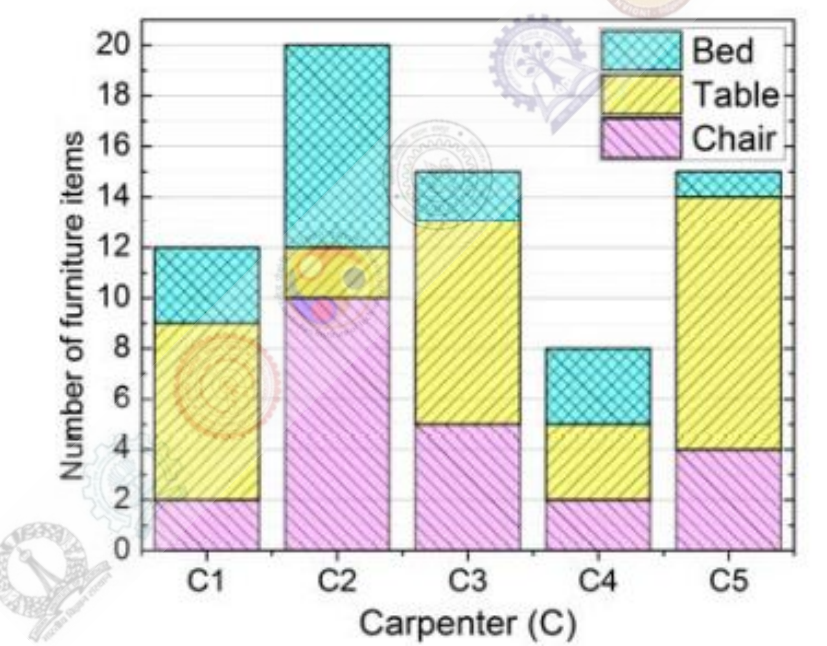
\includegraphics[width=0.5\textwidth]{figs/fig.png}
    \end{figure}
    
    Consider the following statements
    \begin{enumerate}
        \item The number of beds made by carpenter C2 is exactly the same as the number of tables made by carpenter C3.
        \item The total number of chairs made by all carpenters is less than the total number of tables
    \end{enumerate}
    Which one of the following is true?
    \begin{multicols}{4}
        \begin{enumerate}
            \item Only (a)
            \item Only (b)
            \item Both (a) and (b)
            \item Neither (a) nor (b)
        \end{enumerate}
    \end{multicols}
    
\end{enumerate}
\end{document}